\chapter{आयनिक और आण्विक ठोसों का घुलना}\label{ch:g11:dissolution}

पानी में मिलाकर चलाई गई एक चुटकी नमक कुछ ही सेकंड में ग़ायब हो जाती है; वही
चुटकी खाना पकाने के तेल में चलाई जाए तो गिलास की तली में, बिना बदले, तब तक
पड़ी रहती है जब तक कोई देखना चाहे। नल के नीचे धोई गई चिकनी कड़ाही चिकनी ही रहती
है; बर्तन धोने के तरल की एक बूँद, और चिकनाई उतर जाती है। कोई पदार्थ किसी द्रव में
घुलेगा या नहीं, यह क्या तय करता है? उत्तर पिछले अध्याय के \omterm{def:g11:polarity-and-cohesion:polar-bond}{आंशिक आवेशों} और
कणों के बीच के बलों में छिपा है।

\begin{recall}
\omterm{def:g6:solutions-and-solubility:solubility}{विलेयता}; \omterm{def:g6:solutions-and-solubility:miscible}{मिश्रणीय} और \omterm{def:g6:solutions-and-solubility:miscible}{अमिश्रणीय} द्रव
(\cref{ch:g6:solutions-and-solubility})। \omterm{def:g9:ions:ionic-compound}{आयनिक यौगिक} \omterm{def:g9:ions:ion}{धनायनों} और \omterm{def:g9:ions:ion}{ऋणायनों} से
ऐसे अनुपात में बना होता है कि वह उदासीन रहे
(\cref{ch:g9:ions})। ध्रुवीय और \omterm{def:g11:polarity-and-cohesion:polar-molecule}{अध्रुवीय अणु}, \omterm{def:g11:polarity-and-cohesion:hydrogen-bond}{हाइड्रोजन आबंध},
\omterm{def:g11:polarity-and-cohesion:van-der-waals}{वान्डरवाल्स अन्योन्यक्रियाएँ} (\cref{ch:g11:polarity-and-cohesion})।
\omterm{def:g10:chemical-species:extraction}{द्रव--द्रव निष्कर्षण} (\cref{ch:g10:chemical-species})। \omterm{def:g10:concentration-and-dilution:molar-concentration}{मोलर
सांद्रता} (\cref{ch:g10:concentration-and-dilution})।
\end{recall}

\section{आयनिक ठोस का घुलना}

सोडियम क्लोराइड के क्रिस्टल में हर सोडियम \omterm{def:g9:ions:ion}{आयन} \ce{Na+} क्लोराइड \omterm{def:g9:ions:ion}{आयनों} \ce{Cl-}
से घिरा होता है और हर क्लोराइड \omterm{def:g9:ions:ion}{आयन} सोडियम \omterm{def:g9:ions:ion}{आयनों} से, सभी विपरीत आवेशों के बीच के
आकर्षण से जुड़े हुए। पानी के \omterm{def:g11:polarity-and-cohesion:polar-molecule}{ध्रुवीय अणु} इन आवेशों से आकर्षित होते हैं: उनका
ऑक्सीजन वाला सिरा ($\delta^-$) \omterm{def:g9:ions:ion}{धनायनों} की ओर मुड़ता है, हाइड्रोजन वाला सिरा
($\delta^+$) \omterm{def:g9:ions:ion}{ऋणायनों} की ओर।

\begin{definition}[वियोजन]\label{def:g11:dissolution:dissociation}
किसी \omterm{def:g6:solutions-and-solubility:solute}{विलायक} में आयनिक ठोस का \emph{वियोजन}\index{वियोजन} उसके \omterm{def:g9:ions:ion}{आयनों} का एक-दूसरे
से अलग होना है: वे क्रिस्टल छोड़ देते हैं और विलयन में एक-दूसरे से दूर
चले जाते हैं।
\end{definition}

\begin{definition}[विलायकन, जलयोजन]\label{def:g11:dissolution:solvation}
किसी घुले हुए कण का \emph{विलायकन}\index{विलायकन} उसका \omterm{def:g6:solutions-and-solubility:solute}{विलायक} के \omterm{def:g7:atoms-and-molecules:molecule}{अणुओं} से घिर
जाना है, जो आकर्षणों से उससे जुड़े रहते हैं; पानी में इसे
\emph{जलयोजन}\index{जलयोजन} कहते हैं। किसी सूत्र के बाद लिखे संकेत (aq) का अर्थ है
``जलयोजित''।
\end{definition}

\begin{proposition}[घुलने के तीन चरण]\label{prop:g11:dissolution:stages}
आयनिक ठोस पानी में तीन चरणों में \omterm{def:g2:mixing-and-dissolving:dissolve}{घुलता} है जो साथ-साथ होते हैं:
\omterm{def:g9:ions:ion}{आयन} क्रिस्टल से बाहर खींचे जाते हैं (\omterm{def:g11:dissolution:dissociation}{वियोजन}), पानी के \omterm{def:g7:atoms-and-molecules:molecule}{अणुओं} से घिर जाते हैं
(\omterm{def:g11:dissolution:solvation}{जलयोजन}), और पूरे विलयन में फैल जाते हैं
(परिक्षेपण)। सोडियम क्लोराइड के लिए,
\[
  \ce{NaCl(s) -> Na+(aq) + Cl-(aq)} .
\]
\end{proposition}

\begin{proof}
स्वीकृत: \omterm{def:g9:ions:ion}{आयनों} और पानी के \omterm{def:g11:polarity-and-cohesion:polar-molecule}{ध्रुवीय अणुओं} के बीच के आकर्षण, मिलाकर,
इतने प्रबल होते हैं कि वे क्रिस्टल के \omterm{def:g9:ions:ion}{आयनों} के बीच के आकर्षणों की जगह ले
सकें।
\end{proof}

\begin{omfigure}
\begin{tikzpicture}[font=\small]
  % the crystal edge: alternating ions
  \foreach \i in {0,1,2,3,4} \foreach \j in {0,1,2,3} {
    \pgfmathtruncatemacro\k{mod(\i+\j,2)}
    \ifnum\k=0
      \node[om atom, ball color=green!60!black, minimum size=6.4mm] at (0.8*\i,0.8*\j) {};
    \else
      \node[om atom, ball color=violet!70, minimum size=4.0mm] at (0.8*\i,0.8*\j) {};
    \fi
  }
  % a hydrated Na+ that has left: O towards the ion
  \begin{scope}[shift={(5.6,1.8)}]
    \node[om atom, ball color=violet!70, minimum size=4.0mm] (na) at (0,0) {};
    \node[font=\footnotesize] at (0,0) {};
    \foreach \a in {0,90,180,270} {
      \node[aO, minimum size=4.6mm] (o\a) at (\a:0.62) {};
      \node[aH, minimum size=3.2mm] (ha\a) at ($(\a:0.62)+(\a+52:0.42)$) {};
      \node[aH, minimum size=3.2mm] (hb\a) at ($(\a:0.62)+(\a-52:0.42)$) {};
      \begin{scope}[on background layer]
        \draw[bond, line width=1.2pt] (o\a.center) -- (ha\a.center);
        \draw[bond, line width=1.2pt] (o\a.center) -- (hb\a.center);
      \end{scope}
    }
    \node[anchor=north] at (0,-1.35) {\ce{Na+(aq)}};
  \end{scope}
  % a hydrated Cl- that has left: H towards the ion
  \begin{scope}[shift={(8.6,1.4)}]
    \node[om atom, ball color=green!60!black, minimum size=6.4mm] at (0,0) {};
    \foreach \a in {45,135,225,315} {
      \node[aH, minimum size=3.2mm] (h\a) at (\a:0.62) {};
      \node[aO, minimum size=4.6mm] (o\a) at (\a:1.0) {};
      \node[aH, minimum size=3.2mm] (k\a) at ($(\a:1.0)+(\a+75:0.42)$) {};
      \begin{scope}[on background layer]
        \draw[bond, line width=1.2pt] (o\a.center) -- (h\a.center);
        \draw[bond, line width=1.2pt] (o\a.center) -- (k\a.center);
      \end{scope}
    }
    \node[anchor=north] at (0,-1.45) {\ce{Cl-(aq)}};
  \end{scope}
  \node[anchor=north, align=center] at (1.6,-0.45) {क्रिस्टल\\
    (\ce{Na+} छोटा, \ce{Cl-} बड़ा)};
\end{tikzpicture}

{\small सोडियम क्लोराइड का \omterm{def:g2:mixing-and-dissolving:dissolve}{घुलना}। एक सोडियम \omterm{def:g9:ions:ion}{आयन} और एक क्लोराइड \omterm{def:g9:ions:ion}{आयन}
क्रिस्टल छोड़ चुके हैं; हर एक जलयोजित है। \omterm{def:g9:ions:ion}{धनायन} के चारों ओर पानी के \omterm{def:g7:atoms-and-molecules:molecule}{अणु}
अपने ऑक्सीजन \omterm{def:g7:atoms-and-molecules:atom}{परमाणु} (लाल, $\delta^-$) भीतर की ओर मोड़ते हैं, \omterm{def:g9:ions:ion}{ऋणायन} के चारों ओर
अपने हाइड्रोजन \omterm{def:g7:atoms-and-molecules:atom}{परमाणु} (सफ़ेद, $\delta^+$)।}
\end{omfigure}

\section{आयनों की सांद्रताएँ}

\begin{method}[हर आयन की सांद्रता]\label{met:g11:dissolution:ions}
\begin{enumerate}
  \item \omterm{def:g2:mixing-and-dissolving:dissolve}{घुलने} का समीकरण लिखिए, \omterm{def:g7:atoms-and-molecules:atom}{परमाणुओं} और आवेश दोनों में संतुलित:
        कैल्सियम क्लोराइड के लिए \ce{CaCl2(s) -> Ca^{2+}(aq) + 2Cl-(aq)}।
  \item घुले हुए ठोस की मात्रा $n$, और \omterm{def:g6:solutions-and-solubility:solute}{विलेय} में विलयन की सांद्रता
        $c = n / V$, निकालिए।
  \item हर \omterm{def:g9:ions:ion}{आयन} की सांद्रता समीकरण में उसके गुणांक से गुणा की गई $c$ है:
        यहाँ $[\ce{Ca^{2+}}] = c$ और
        $[\ce{Cl-}] = 2c$।
\end{enumerate}
वर्ग कोष्ठक $[\ldots]$ किसी घुली हुई स्पीशीज़ की \omterm{def:g10:concentration-and-dilution:molar-concentration}{मोलर सांद्रता}
दर्शाते हैं।
\end{method}

\begin{example}[कैल्सियम क्लोराइड]\label{ex:g11:dissolution:cacl2}
% ledger: aw:Ca, aw:Cl
पानी में \qty{5.55}{g} कैल्सियम क्लोराइड ($M = \qty{111.1}{g/mol}$) घोलकर
\qty{500.0}{mL} विलयन बनाया जाता है: $n = \qty{0.0500}{mol}$,
$c = \qty{0.100}{mol/L}$, इसलिए $[\ce{Ca^{2+}}] = \qty{0.100}{mol/L}$ और
$[\ce{Cl-}] = \qty{0.200}{mol/L}$। विलयन उदासीन है: प्रति लीटर $2 \times
0.100$ धनात्मक आवेश, और $1 \times 0.200$ ऋणात्मक।
\end{example}

\section{ध्रुवता और विलेयता}

\begin{proposition}[समान, समान को घोलता है]\label{prop:g11:dissolution:like}
पानी जैसा ध्रुवीय \omterm{def:g6:solutions-and-solubility:solute}{विलायक} आयनिक ठोसों और ध्रुवीय
स्पीशीज़ को घोलता है, विशेषकर उन्हें जो उसके साथ \omterm{def:g11:polarity-and-cohesion:hydrogen-bond}{हाइड्रोजन आबंध} बना सकती हैं;
साइक्लोहेक्सेन या वनस्पति तेल जैसा अध्रुवीय \omterm{def:g6:solutions-and-solubility:solute}{विलायक} अध्रुवीय स्पीशीज़ को
घोलता है। आयनिक ठोस अध्रुवीय \omterm{def:g6:solutions-and-solubility:solute}{विलायकों} में बहुत कम \omterm{def:g2:mixing-and-dissolving:dissolve}{घुलते} हैं, और
अध्रुवीय स्पीशीज़ पानी में बहुत कम।
\end{proposition}

\begin{proof}
स्वीकृत: कोई \omterm{def:g6:solutions-and-solubility:solute}{विलेय} तब अच्छी तरह \omterm{def:g2:mixing-and-dissolving:dissolve}{घुलता} है जब \omterm{def:g6:solutions-and-solubility:solute}{विलायक} के साथ वह जो आकर्षण बना
सकता है, वे कम से कम उतने प्रबल हों जितने वह तोड़ता है, अपने कणों के बीच
और \omterm{def:g6:solutions-and-solubility:solute}{विलायक} के \omterm{def:g7:atoms-and-molecules:molecule}{अणुओं} के बीच।
\end{proof}

\begin{example}[तीन स्थितियाँ]\label{ex:g11:dissolution:cases}
% ledger: sol:I2-water, sol:I2-heptane
एथेनॉल पानी में हर अनुपात में मिल जाता है: उसका \ce{O-H} समूह पानी के साथ
\omterm{def:g11:polarity-and-cohesion:hydrogen-bond}{हाइड्रोजन आबंध} बनाता है। नमक पानी में \omterm{def:g2:mixing-and-dissolving:dissolve}{घुलता} है पर तेल में नहीं।
आयोडीन, \ce{I2}, एक \omterm{def:g11:polarity-and-cohesion:polar-molecule}{अध्रुवीय अणु}, पानी में कम \omterm{def:g2:mixing-and-dissolving:dissolve}{घुलता} है (लगभग
\qty{0.3}{g/L}, एक भूरा विलयन) पर अध्रुवीय \omterm{def:g6:solutions-and-solubility:solute}{विलायकों} में अच्छी तरह
(प्रति किलोग्राम हेप्टेन \qty{17}{g}, एक बैंगनी विलयन)।
\end{example}

\section{द्रव--द्रव निष्कर्षण, समझाया गया}

\omterm{def:g10:chemical-species:extraction}{द्रव--द्रव निष्कर्षण} किसी स्पीशीज़ को एक \omterm{def:g6:solutions-and-solubility:solute}{विलायक} से ऐसे दूसरे \omterm{def:g6:solutions-and-solubility:solute}{विलायक} में ले जाता
है जो पहले के साथ \omterm{def:g6:solutions-and-solubility:miscible}{अमिश्रणीय} हो और जिसमें वह अधिक \omterm{def:g6:solutions-and-solubility:solute}{विलेय} हो। नियम
``समान, समान को घोलता है'' बताता है कि कौन-सा \omterm{def:g6:solutions-and-solubility:solute}{विलायक} चुनना है।

\begin{inthelab}[आयोडीन का निष्कर्षण]
भूरे जलीय आयोडीन विलयन का \qty{20}{mL} एक पृथक्कारी कीप में
\qty{10}{mL} साइक्लोहेक्सेन के साथ डाला जाता है। कीप को डाट से बंद करके
हिलाया जाता है, टोंटी से उसका दाब निकाला जाता है, और उसे ठहरने के लिए छोड़ दिया
जाता है। दो परतें बनती हैं: कम घना साइक्लोहेक्सेन ऊपर। ऊपरी परत
अब बैंगनी है, निचली लगभग रंगहीन: आयोडीन साइक्लोहेक्सेन में चला गया
है। निचली परत टोंटी से निकाल दी जाती है, और
आयोडीन साइक्लोहेक्सेन में वापस मिल जाता है।
\end{inthelab}

\begin{omfigure}
\begin{tikzpicture}[font=\small, scale=1.15]
  \pic[transform shape] at (0,0) {sepfunnel={orange!55!brown!70}{white}};
  \node[anchor=north, align=center] at (0,-0.15) {हिलाने से पहले};
  \draw[omProp, <-] (0.55,2.1) -- (1.4,2.5) node[right, text=black] {साइक्लोहेक्सेन};
  \draw[omProp, <-] (0.45,1.35) -- (1.4,1.2) node[right, text=black,
    align=left] {जलीय\\ आयोडीन (भूरा)};
  \pic[transform shape] at (4.6,0) {sepfunnel={orange!10}{violet!60}};
  \node[anchor=north, align=center] at (4.6,-0.15) {हिलाने और ठहरने\\ के बाद};
  \draw[omProp, <-] (5.15,2.1) -- (6.0,2.5) node[right, text=black,
    align=left] {साइक्लोहेक्सेन में\\ आयोडीन (बैंगनी)};
  \draw[omProp, <-] (5.05,1.35) -- (6.0,1.2) node[right, text=black,
    align=left] {पानी, लगभग\\ रंगहीन};
\end{tikzpicture}

{\small साइक्लोहेक्सेन से पानी में से आयोडीन का \omterm{def:g10:chemical-species:extraction}{निष्कर्षण}। अध्रुवीय आयोडीन
अध्रुवीय \omterm{def:g6:solutions-and-solubility:solute}{विलायक} में चला जाता है; पानी से कम घना साइक्लोहेक्सेन
ऊपर तैरता है।}
\end{omfigure}

\begin{safety}{\ghs[0.82cm]{GHS02}\ghs[0.82cm]{GHS07}\ghs[0.82cm]{GHS08}\ghs[0.82cm]{GHS09}}
% ledger: ghs:I2, ghs:cyclohexane
साइक्लोहेक्सेन अत्यधिक ज्वलनशील है, इसकी वाष्प उनींदापन लाती है, निगलने पर यह
फेफड़ों के लिए हानिकारक है और जलीय जीवों के लिए अत्यंत विषैला है। आयोडीन
त्वचा के संपर्क से और साँस में लेने पर हानिकारक है। धूम-हुड, चश्मा और
दस्ताने, पास में कहीं कोई लौ नहीं; कार्बनिक अपशिष्ट इकट्ठा किया जाता है।
\end{safety}


\section{साबुन और उभयरागी अणु}

\begin{definition}[जलरागी, जलविरागी]\label{def:g11:dissolution:hydrophilic}
कोई स्पीशीज़ या \omterm{def:g7:atoms-and-molecules:molecule}{अणु} का कोई भाग \emph{जलरागी}\index{जलरागी} होता है
अगर वह पानी से आकर्षित हो (आयनिक या ध्रुवीय समूह, \omterm{def:g11:polarity-and-cohesion:hydrogen-bond}{हाइड्रोजन आबंध} बनाने वाले
समूह); वह \emph{जलविरागी}\index{जलविरागी} होता है अगर ऐसा न हो
(कार्बन और हाइड्रोजन \omterm{def:g7:atoms-and-molecules:atom}{परमाणुओं} की लंबी, अध्रुवीय श्रृंखलाएँ)। जलविरागी
स्पीशीज़ वसाओं और तेलों में \omterm{def:g2:mixing-and-dissolving:dissolve}{घुलती} हैं।
\end{definition}

\begin{definition}[उभयरागी अणु, मिसेल]\label{def:g11:dissolution:amphiphilic}
\emph{उभयरागी}\index{उभयरागी} \omterm{def:g7:atoms-and-molecules:molecule}{अणु} या \omterm{def:g9:ions:ion}{आयन} का एक \omterm{def:g11:dissolution:hydrophilic}{जलरागी} सिर और एक
\omterm{def:g11:dissolution:hydrophilic}{जलविरागी} पूँछ होती है। पानी में उभयरागी \omterm{def:g9:ions:ion}{आयन}
\emph{मिसेलों}\index{मिसेल} में इकट्ठे हो जाते हैं: नन्हे गोले, जिनमें पूँछें
भीतर, पानी से बाहर, और सिर सतह पर, पानी के संपर्क में
होते हैं।
\end{definition}

\begin{example}[एक साबुन]\label{ex:g11:dissolution:soap}
% ledger: aw:C, aw:H, aw:O, aw:Na
सोडियम स्टीयरेट, \ce{C17H35COONa} ($M = \qty{306.0}{g/mol}$), एक
विशिष्ट साबुन है, जो जंतु या वनस्पति वसाओं से बनता है। पानी में वह
सोडियम \omterm{def:g9:ions:ion}{आयनों} \ce{Na+} और स्टीयरेट \omterm{def:g9:ions:ion}{आयनों} \ce{C17H35COO-} के रूप में \omterm{def:g2:mixing-and-dissolving:dissolve}{घुलता} है: एक सिर
\ce{-COO-}, आयनिक, \omterm{def:g11:dissolution:hydrophilic}{जलरागी}, और 17 कार्बन \omterm{def:g7:atoms-and-molecules:atom}{परमाणुओं} की एक पूँछ,
\omterm{def:g11:dissolution:hydrophilic}{जलविरागी}।
\end{example}

\begin{omfigure}
\begin{tikzpicture}[font=\small]
  % the stearate ion as a zigzag of 17 carbons + COO-
  \foreach \k in {0,1,2,3,4,5,6,7,8,9,10,11,12,13,14,15,16} {
    \pgfmathsetmacro\y{mod(\k,2)==0 ? 0 : 0.3}
    \coordinate (c\k) at (0.42*\k,\y);
  }
  \draw[line width=0.9pt] (c0) \foreach \k in {1,2,3,4,5,6,7,8,9,10,11,12,13,14,15,16} { -- (c\k) };
  \coordinate (cc) at ($(c16)+(30:0.42)$);
  \begin{scope}[on background layer]
    \fill[omDef!15, rounded corners] ($(cc)+(-0.25,-0.55)$) rectangle ($(cc)+(1.05,0.9)$);
  \end{scope}
  \draw[line width=0.9pt] (c16) -- (cc);
  \draw[line width=0.9pt] (cc) -- ++(90:0.4) node[above] {O};
  \draw[line width=0.9pt] ([xshift=1.5pt]cc) -- ++(90:0.36);
  \draw[line width=0.9pt] (cc) -- ++(-30:0.42) node[right] {O$^-$};
  \draw[omProp] ($(c0)+(0,-0.15)$) -- ++(0,-0.15) -- ($(c16)+(0,-0.3)$) -- ++(0,0.15);
  \node[omProp, anchor=north] at ($(c8)+(0,-0.32)$) {जलविरागी पूँछ (17 कार्बन परमाणु)};
  \node[omDef, anchor=south] at ($(cc)+(0.35,0.9)$) {जलरागी सिर};
  % the sketch
  \begin{scope}[yshift=-1.9cm]
    \draw[omProp, line width=1.6pt, decorate, decoration={snake, amplitude=1.5pt,
      segment length=6pt}] (2.0,0) -- (5.2,0);
    \fill[omDef] (5.45,0) circle (0.25);
    \node[white, font=\scriptsize\bfseries] at (5.45,0) {$-$};
    \node[anchor=west] at (5.9,0) {वही आयन, रेखाचित्र में};
  \end{scope}
\end{tikzpicture}

{\small स्टीयरेट \omterm{def:g9:ions:ion}{आयन}। इस टेढ़े-मेढ़े चित्र में श्रृंखला का हर कोना एक कार्बन
\omterm{def:g7:atoms-and-molecules:atom}{परमाणु} है जिस पर हाइड्रोजन \omterm{def:g7:atoms-and-molecules:atom}{परमाणु} हैं (\ce{CH2}, और सिरे पर \ce{CH3});
आगे का एक अध्याय यह संक्षिप्त रूप समझाता है। नीचे, सामान्य
रेखाचित्र: लहरदार पूँछ और गोल सिर।}
\end{omfigure}

\begin{proposition}[साबुन चिकनाई कैसे हटाता है]\label{prop:g11:dissolution:soap}
चिकनाई \omterm{def:g11:dissolution:hydrophilic}{जलविरागी} है और पानी में नहीं \omterm{def:g2:mixing-and-dissolving:dissolve}{घुलती}। साबुन वाले पानी में
साबुन के \omterm{def:g9:ions:ion}{आयनों} की पूँछें चिकनाई में घुल जाती हैं जबकि सिर पानी में रहते
हैं; चिकनाई नन्ही बूँदों में टूट जाती है, हर बूँद एक ऐसे \omterm{def:g11:dissolution:amphiphilic}{मिसेल} में लिपटी होती है
जिसकी आवेशित सतह पानी की ओर होती है, और बूँदें
धोने वाले पानी के साथ बह जाती हैं।
\end{proposition}

\begin{proof}
स्वीकृत: यह \omterm{def:g9:ions:ion}{आयन} के हर सिरे पर ``समान, समान को घोलता है'' लागू करने से निकलता
है; बाहर के आवेशित सिर बूँदों को फिर से आपस में मिलने से भी रोकते हैं,
क्योंकि समान आवेश एक-दूसरे को प्रतिकर्षित करते हैं।
\end{proof}

\begin{omfigure}
\begin{tikzpicture}[font=\small]
  \fill[yellow!45!orange!35] (0,0) circle (1.0);
  \node at (0,0) {चिकनाई};
  \foreach \a in {0,20,40,60,80,100,120,140,160,180,200,220,240,260,280,300,320,340} {
    \draw[omProp, line width=1.3pt, decorate, decoration={snake,
      amplitude=1pt, segment length=4pt}] (\a:0.55) -- (\a:1.45);
    \fill[omDef] (\a:1.6) circle (0.15);
  }
  \node[anchor=west, align=left] at (2.4,0.6) {सिर ($-$) पानी में};
  \node[anchor=west, align=left] at (2.4,-0.4) {पूँछें चिकनाई में};
  \draw[black!50] (2.4,0.6) -- (1.75,0.45);
  \draw[black!50] (2.4,-0.4) -- (1.05,-0.25);
  \node[font=\small, blue!50!black] at (-2.6,1.4) {पानी};
\end{tikzpicture}

{\small अनुप्रस्थ काट में एक \omterm{def:g11:dissolution:amphiphilic}{मिसेल}: चिकनाई की एक बूँद के चारों ओर साबुन के \omterm{def:g9:ions:ion}{आयन},
पूँछें भीतर, आवेशित सिर बाहर। हर \omterm{def:g11:dissolution:amphiphilic}{मिसेल} की सतह ऋणावेशित होती है,
और \omterm{def:g11:dissolution:amphiphilic}{मिसेल} एक-दूसरे को प्रतिकर्षित करते हैं।}
\end{omfigure}

\begin{omfigure}
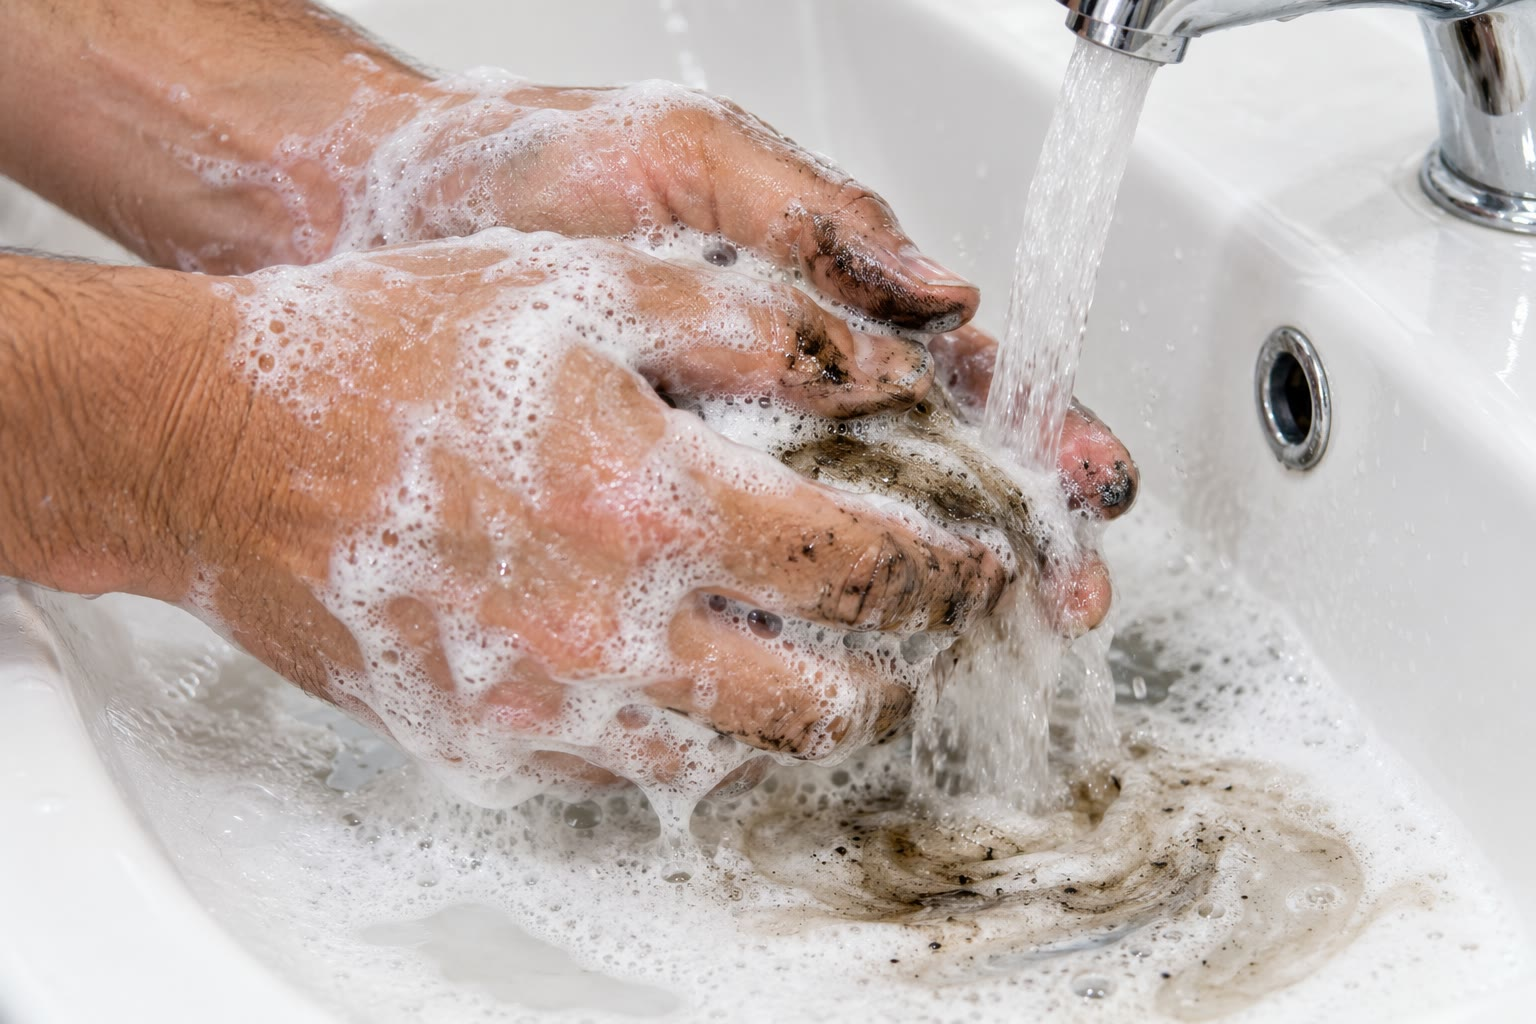
\includegraphics[width=0.48\linewidth]{images/book1/ai/g11-greasy-hands.jpg}

{\small चिकने हाथ धोना: साबुन चिकनाई को \omterm{def:g11:dissolution:amphiphilic}{मिसेलों} में बहा ले जाता है।}
\end{omfigure}

\begin{remark}[कठोर पानी और मैल]\label{rem:g11:dissolution:scum}
कठोर पानी में बहुत-से कैल्सियम \omterm{def:g9:ions:ion}{आयन} \ce{Ca^{2+}} और मैग्नीशियम \omterm{def:g9:ions:ion}{आयन}
\ce{Mg^{2+}} होते हैं, जो उन चट्टानों से घुलकर आते हैं जिनसे होकर वह बहा है। स्टीयरेट
\omterm{def:g9:ions:ion}{आयनों} के साथ वे एक \omterm{def:g9:ions:precipitate}{अवक्षेप} (\cref{ch:g9:ions}), कैल्सियम स्टीयरेट, बनाते हैं:
\[
  \ce{2C17H35COO- + Ca^{2+} -> Ca(C17H35COO)2(s)} .
\]
यही धूसर ठोस वह मैल है जो वॉशबेसिन में छल्ला बनाता है, और उसमें फँसा साबुन का हर
\omterm{def:g9:ions:ion}{आयन} धोने के काम से निकल जाता है: कठोर पानी में साबुन ठीक से झाग नहीं देता,
जब तक इतना न मिला दिया जाए कि सारा कैल्सियम अवक्षेपित हो जाए।
\end{remark}

\begin{omfigure}
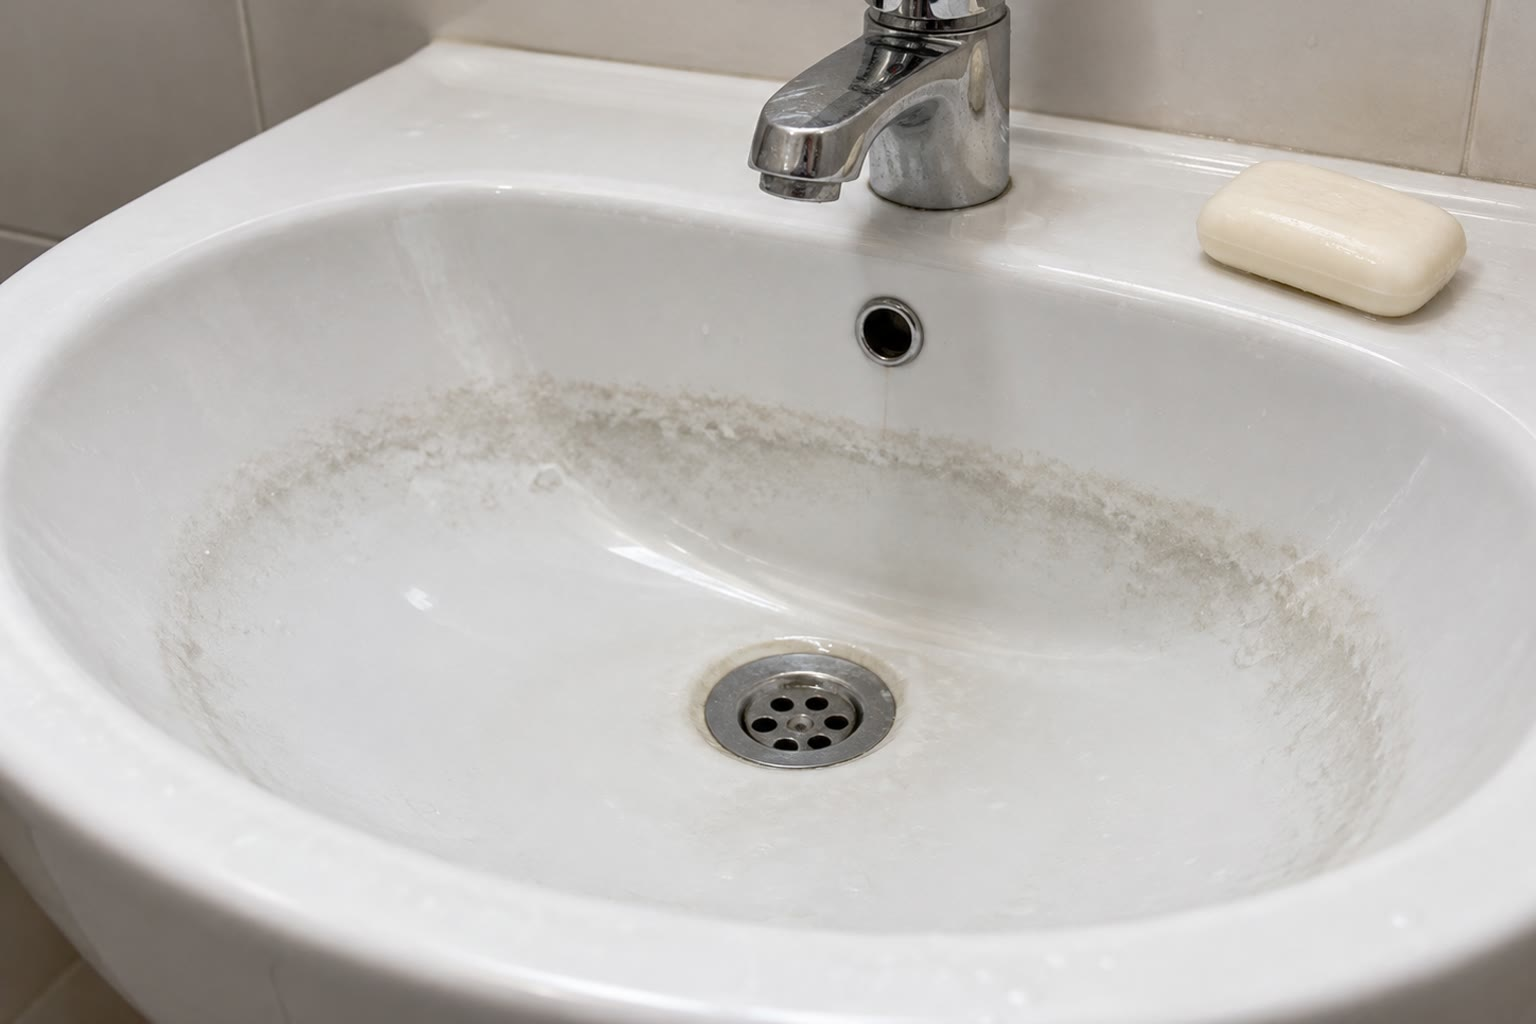
\includegraphics[width=0.45\linewidth]{images/book1/ai/g11-soap-scum.jpg}

{\small वॉशबेसिन में साबुन का मैल: कठोर पानी द्वारा अवक्षेपित
कैल्सियम स्टीयरेट।}
\end{omfigure}

\section{अभ्यास}


\begin{exercise}[$\star$]\label{exo:g11:dissolution:1}
सोडियम क्लोराइड \ce{NaCl}, कैल्सियम क्लोराइड \ce{CaCl2}, सोडियम सल्फ़ेट
\ce{Na2SO4} और ऐलुमिनियम क्लोराइड \ce{AlCl3} के पानी में \omterm{def:g2:mixing-and-dissolving:dissolve}{घुलने} के समीकरण
लिखिए।
\end{exercise}

\begin{exercise}[$\star$]\label{exo:g11:dissolution:2}
सोडियम सल्फ़ेट के एक विलयन का $c = \qty{0.050}{mol/L}$ है। सोडियम \omterm{def:g9:ions:ion}{आयनों} और
सल्फ़ेट \omterm{def:g9:ions:ion}{आयनों} की सांद्रताएँ बताइए।
\end{exercise}

\begin{exercise}[$\star$]\label{exo:g11:dissolution:3}
किसी \omterm{def:g9:ions:ion}{आयन} के \omterm{def:g11:dissolution:solvation}{जलयोजन} का क्या अर्थ है? पानी के \omterm{def:g7:atoms-and-molecules:molecule}{अणु} का कौन-सा सिरा \omterm{def:g9:ions:ion}{धनायन} की ओर,
और कौन-सा \omterm{def:g9:ions:ion}{ऋणायन} की ओर रहता है? क्यों?
\end{exercise}

\begin{exercise}[$\star$]\label{exo:g11:dissolution:4}
\qty{2.67}{g} ऐलुमिनियम क्लोराइड घोलकर \qty{200.0}{mL} विलयन बनाया जाता है।
विलयन की और हर \omterm{def:g9:ions:ion}{आयन} की सांद्रता
निकालिए।
\end{exercise}

\begin{exercise}[$\star$]\label{exo:g11:dissolution:5}
स्टीयरेट \omterm{def:g9:ions:ion}{आयन} के हर भाग को \omterm{def:g11:dissolution:hydrophilic}{जलरागी} या \omterm{def:g11:dissolution:hydrophilic}{जलविरागी} के रूप में चिह्नित कीजिए, और
बताइए क्यों।
\end{exercise}

\begin{exercise}[$\star\star$]\label{exo:g11:dissolution:6}
इन्हें घोलने के लिए आप कौन-सा \omterm{def:g6:solutions-and-solubility:solute}{विलायक}, पानी या साइक्लोहेक्सेन, चुनेंगे: नमक;
मोमबत्ती का मोम (लंबी हाइड्रोकार्बन श्रृंखलाएँ); चीनी (बहुत-से \ce{O-H} समूह);
आयोडीन? हर चुनाव का औचित्य बताइए।
\end{exercise}

\begin{exercise}[$\star\star$]\label{exo:g11:dissolution:7}
एथेनॉल \ce{CH3-CH2-OH} पानी में हर अनुपात में मिल जाता है, पर हेक्सेन
\ce{C6H14} पानी में नहीं मिलता। समझाइए।
\end{exercise}

\begin{exercise}[$\star\star$]\label{exo:g11:dissolution:8}
\omterm{def:g11:dissolution:amphiphilic}{मिसेल} वाला चित्र देखिए। पूँछें भीतर और सिर बाहर क्यों हैं? दो \omterm{def:g11:dissolution:amphiphilic}{मिसेल}
मिलकर चिकनाई की एक बड़ी बूँद क्यों नहीं बन जाते?
\end{exercise}

\begin{exercise}[$\star\star$]\label{exo:g11:dissolution:9}
किसी पौधे की सुगंध पानी में घुली है। उसके \omterm{def:g10:chemical-species:extraction}{निष्कर्षण} के लिए रसायनज्ञ
एथेनॉल या साइक्लोहेक्सेन का उपयोग कर सकता है। कौन-सा उपयुक्त है, और दूसरा क्यों
नहीं (मिश्रणीयता के बारे में सोचिए)?
\end{exercise}

\begin{exercise}[$\star\star$]\label{exo:g11:dissolution:10}
आयोडीन के \omterm{def:g10:chemical-species:extraction}{निष्कर्षण} में साइक्लोहेक्सेन की परत ऊपर क्यों है? कौन-सी
परत टोंटी से निकाली जाती है? अंत में आयोडीन कहाँ है?
\end{exercise}

\begin{exercise}[$\star\star$]\label{exo:g11:dissolution:11}
कॉपर सल्फ़ेट के नीले विलयन को साइक्लोहेक्सेन के साथ हिलाया जाता है। नीले रंग का
क्या होता है? समझाइए।
\end{exercise}

\begin{exercise}[$\star\star\star$]\label{exo:g11:dissolution:12}
$[\ce{Cl-}] = \qty{0.300}{mol/L}$ वाला \qty{250.0}{mL} विलयन बनाने के लिए
कैल्सियम क्लोराइड का कितना द्रव्यमान घोलना होगा?
\end{exercise}

\begin{exercise}[$\star\star\star$]\label{exo:g11:dissolution:13}
समुद्र के पानी के एक नमूने में \qty{0.010}{mol/L} कैल्सियम
\omterm{def:g9:ions:ion}{आयन} और \qty{0.053}{mol/L} मैग्नीशियम \omterm{def:g9:ions:ion}{आयन} पाए जाते हैं। समझाइए कि साधारण साबुन
समुद्र के पानी में बहुत ख़राब झाग क्यों देता है। एक लीटर समुद्र के पानी के केवल
कैल्सियम \omterm{def:g9:ions:ion}{आयन} कितना सोडियम स्टीयरेट अवक्षेपित करेंगे?
\end{exercise}

\begin{exercise}[$\star\star\star$]\label{exo:g11:dissolution:14}
\qty{0.20}{mol/L} वाले सोडियम क्लोराइड विलयन का \qty{100.0}{mL}
\qty{0.10}{mol/L} वाले कैल्सियम क्लोराइड विलयन के \qty{100.0}{mL} के साथ
मिलाया जाता है। कोई \omterm{def:g9:ions:precipitate}{अवक्षेप} नहीं बनता। \omterm{def:g6:pure-substances-and-mixtures:mixture}{मिश्रण} में
\ce{Na+}, \ce{Ca^{2+}} और \ce{Cl-} की सांद्रताएँ निकालिए, और जाँचिए कि वह
उदासीन है।
\end{exercise}

\begin{exercise}[$\star\star\star$]\label{exo:g11:dissolution:15}
% ledger: sol:I2-water, sol:I2-heptane, rho:heptane
आयोडीन प्रति लीटर पानी लगभग \qty{0.3}{g} और प्रति किलोग्राम हेप्टेन
\qty{17}{g} \omterm{def:g2:mixing-and-dissolving:dissolve}{घुलता} है। हेप्टेन का घनत्व लगभग
\qty{0.68}{kg/L} है। एक लीटर हेप्टेन एक लीटर पानी की तुलना में कितने गुना अधिक
आयोडीन रख सकता है? \omterm{def:g10:chemical-species:extraction}{निष्कर्षण} के लिए इसका क्या अर्थ है?
\end{exercise}

\section{समस्या: साबुन और कठोर पानी}

\begin{problem}[{सप्ताहांत समस्या --- कठोर पानी का एक स्नान कितना साबुन
मैल के रूप में बर्बाद करता है?}]
\label{pb:g11:dissolution:1}
% ledger: aw:Ca, aw:Mg, aw:C, aw:H, aw:O, aw:Na
एक नल के पानी में प्रति लीटर \qty{120}{mg} कैल्सियम \omterm{def:g9:ions:ion}{आयन} और \qty{24}{mg}
मैग्नीशियम \omterm{def:g9:ions:ion}{आयन} हैं। उससे \qty{150}{L} का एक स्नान-टब भरा जाता है, और
नहाने वाला सोडियम स्टीयरेट, \ce{C17H35COONa}, से बना साबुन इस्तेमाल करता है।

\medskip
\noindent\textbf{भाग I --- पानी में क्या है।}
\begin{enumerate}
  \item नल के पानी के कैल्सियम और मैग्नीशियम \omterm{def:g9:ions:ion}{आयन} कहाँ से आते हैं?
  \item कैल्सियम \omterm{def:g9:ions:ion}{आयनों} और मैग्नीशियम \omterm{def:g9:ions:ion}{आयनों} की \omterm{def:g10:concentration-and-dilution:molar-concentration}{मोलर
        सांद्रताएँ} निकालिए।
  \item कैल्सियम \omterm{def:g9:ions:ion}{आयनों} के साथ हाइड्रोजनकार्बोनेट \omterm{def:g9:ions:ion}{आयन},
        \ce{HCO3-}, होते हैं, मानो कैल्सियम हाइड्रोजनकार्बोनेट \ce{Ca(HCO3)2}
        घोला गया हो। \omterm{def:g2:mixing-and-dissolving:dissolve}{घुलने} का वह समीकरण लिखिए, और कैल्सियम के साथ आने वाले
        हाइड्रोजनकार्बोनेट \omterm{def:g9:ions:ion}{आयनों} की सांद्रता
        निकालिए।
  \item टब में कैल्सियम \omterm{def:g9:ions:ion}{आयनों} की कितनी मात्रा है?
\end{enumerate}

\medskip
\noindent\textbf{भाग II --- साबुन।}
\begin{enumerate}[resume]
  \item सोडियम स्टीयरेट का \omterm{def:g10:the-mole:molar-mass}{मोलर द्रव्यमान} निकालिए।
  \item पानी में उसके \omterm{def:g2:mixing-and-dissolving:dissolve}{घुलने} का समीकरण लिखिए।
  \item स्टीयरेट \omterm{def:g9:ions:ion}{आयन} का कौन-सा भाग \omterm{def:g11:dissolution:hydrophilic}{जलरागी} है, कौन-सा
        \omterm{def:g11:dissolution:hydrophilic}{जलविरागी}? इसे \omterm{def:g11:dissolution:amphiphilic}{उभयरागी} क्यों कहते हैं?
  \item \omterm{def:g11:dissolution:amphiphilic}{मिसेल} का वर्णन कीजिए, और समझाइए कि वह त्वचा से चिकनाई कैसे
        हटाता है।
  \item धोने के लिए साबुन को तेल में नहीं, पानी में क्यों घोलना चाहिए?
\end{enumerate}

\medskip
\noindent\textbf{भाग III --- मैल।}
\begin{enumerate}[resume]
  \item कैल्सियम स्टीयरेट के \omterm{def:g9:ions:precipitate}{अवक्षेपण} का समीकरण लिखिए।
        जाँचिए कि वह आवेश में संतुलित है।
  \item नल के पानी के \qty{1.00}{L} और स्टीयरेट \omterm{def:g9:ions:ion}{आयनों} के
        आधिक्य के लिए \omterm{def:g10:reaction-progress-table:extent}{प्रगति सारणी} भरिए। कौन-सा \omterm{def:g7:chemical-reactions:reactant}{अभिकारक} सीमांत है?
  \item प्रति लीटर स्टीयरेट \omterm{def:g9:ions:ion}{आयनों} की कितनी मात्रा कैल्सियम के कारण खो जाती है?
  \item कैल्सियम स्टीयरेट का \omterm{def:g10:the-mole:molar-mass}{मोलर द्रव्यमान}, और प्रति लीटर बने मैल का द्रव्यमान,
        निकालिए।
  \item मैग्नीशियम स्टीयरेट भी इसी तरह अवक्षेपित होता है। मैग्नीशियम \omterm{def:g9:ions:ion}{आयन} प्रति लीटर
        स्टीयरेट की कितनी मात्रा ले लेते हैं?
\end{enumerate}

\medskip
\noindent\textbf{भाग IV --- स्नान।}
\begin{enumerate}[resume]
  \item पूरे टब का कैल्सियम स्टीयरेट \omterm{def:g9:ions:ion}{आयनों} की कितनी मात्रा
        अवक्षेपित करता है?
  \item यह साबुन का कितना द्रव्यमान है?
  \item मैग्नीशियम जोड़कर, कुल कितना साबुन बर्बाद होता है?
  \item साबुन की टिकियों का भार लगभग \qty{100}{g} होता है। अकेला कैल्सियम कितनी
        टिकियाँ ले लेता है?
  \item अंतिम उत्तर बताइए: इस पानी के \qty{150}{L} के एक स्नान का कैल्सियम
        मैल के रूप में साबुन का कितना द्रव्यमान बर्बाद करता है?
\end{enumerate}
\end{problem}
